\documentclass[../thesis.tex]{subfiles}
\begin{document}
\chapter{Method}\label{cap:methods}
To fulfill the requirements of the project, I adopted an experimental approach. First and foremost, I analyzed the problem in order to understand which kind of sub-problems I was supposed to solve. From that, I was able to determine which tools would have been the most appropriate for doing the computer vision and machine learning tasks and the integration with \gls{ROS}. Then, to experiment with the solution proposed, I designed and developed a proof of concept capable of recognizing and learning a users’ hand gestures and communicating to a robot which action to perform based on the gesture recognized.

\section{Preliminary study}
In analyzing the problem, the following sub-problems emerged to be solved:
\begin{itemize}
    \item a way to capture webcam's frames;
    \item a way to recognize hand gestures, both static and dynamic from the frames received from a webcam;
    \item a way to teach to the system new gestures and connect them to new actions;
    \item a way to convert the recognized gestures into commands for a robot using \gls{ROS} as message exchange system. In particular a way to exchange general purpose messages and set navigation goals;
    \item a way to simulate the proposed solution in different environments.
\end{itemize}

\section{Choice of technologies and tools}\label{sec:technologies_and_tolls}
To achieve goals described above, I decided to use specific technologies and tools available for everyone. The taken decisions have been made based on my knowledge of the technologies and on the necessity to use some specific tools to fulfill the requirements.
\subsection{Python}
Python is a high-level programming language. It is a well-known and highly supported programming language for machine learning tasks. Moreover, it is also supported by \acrshort{ROS} whose documentation has sections written for it. The version used for this project is 3.8 because it is the version distributed within the latest release of Ubuntu operating system. However, being able to use the latest version would allow the exploitation of new statements, for example the pattern matching offered through the \texttt{match ... case} statement, that would make the implementation easier.

\subsection{Tensorflow}
Tensorflow is an open-source Python library to build \acrshort{ML} models. Google began developing it in 2015, and it is now one of the most widely-used Python libraries for performing \acrshort{ML} tasks. It offers a huge number of layers, activation functions, and tools to build simple and complex neural network architectures. The best-known counterpart is PyTorch. During my studies, I have had to use both, and I think Tensorflow is more suitable to develop neural networks oriented toward an application. Instead, PyTorch is more appropriate for the development of new and complex neural networks. Moreover, Tensorflow is better integrated with data collection tools like Tensorboard. 

\subsubsection{Tensorflow lite}
Tensorflow Lite is a component of Tensorflow that allows you to convert a Tensorflow model into a compressed flat buffer and then deploy it onto any device (e.g. mobile devices or embedded devices). With the aim to deploy the hand gesture recognizer to an embedded device like the Nvidia Jetson or distribute it to other people, the use of this tool is natural.

\subsubsection{Keras}
Keras takes advantage of Tensorflow to give the users a powerful API to design and develop Deep Neural Networks. With a few lines of code, it is possible to implement complex neural networks that exploit the latest research in the field of  \gls{ML}.

\subsection{MediaPipe}\label{sec:mediapipe}
MediaPipe is an open-source, real-time, and on-device tool that can track multiple parts of the body. In particular, I am interested in hand tracking. MediaPipe suits very well for this purpose because it offers a pre-trained \acrshort{ML} model to recognize and track twenty-one landmarks on each hand (figure~\ref{fig:landmarksMediapipe}). In particular, it uses a pipeline composed of two \acrshort{ML} models:
\begin{enumerate}
    \item a palm detector that works on a full image locates the palm and identifies the bounding box around it;
    \item a hand landmark model that works on the cropped image of the palm and returns the hand landmarks considering the depth also. That means it can track a landmark behind another one.
\end{enumerate}
\begin{figure}[H]
    \centering
    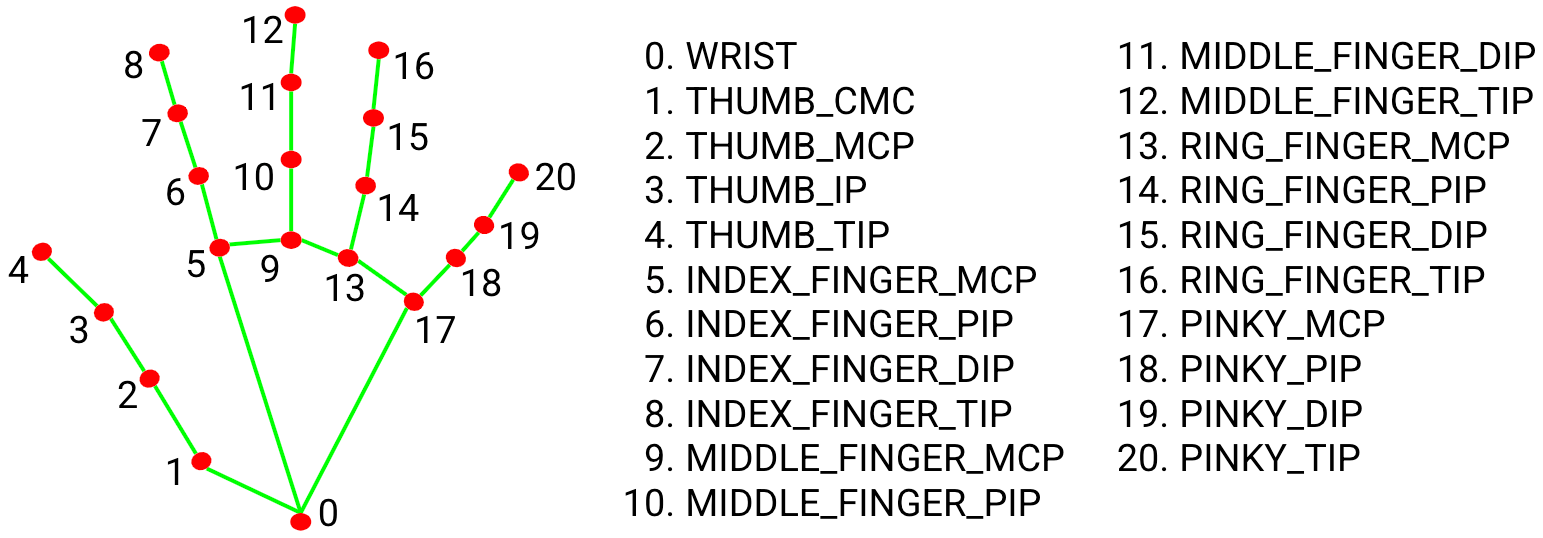
\includegraphics[width=\columnwidth]{thesis/images/mediapipeHandLandmarks.png}
    \caption{Landmarks on a hand recognized by MediaPipe~\cite{site:mediapipe}}
    \label{fig:landmarksMediapipe}
\end{figure}
The precision of this tool is about $96\%$~\cite{paper:mediapipe}, so it is a good starting point for the hand gesture recognition task. It is possible to get the position of the landmarks and give them input through a deep neural network trained on the gestures of our interest. \\
The list of coordinates relatives at position of the hand's landmarks is returned by MediaPipe. These coordinates can be saved and used to train a deep neural network instead of images. This is interesting because: 
\begin{itemize}
    \item it reduces the size of the dataset;
    \item it eliminates environmental factors such as background, lighting, and skin color.
\end{itemize}

It is interesting to point out that MediaPipe is capable of tracking, in real-time, different parts of the human body, for example, the face and the whole body~\cite{site:mediapipe}.

\subsection{OpenCV}
OpenCV is an open-source library that fully meets the requirements regarding computer vision and works well with MediaPipe. It is also distributed as a Python package to integrate into users' applications. 

\subsection{Robot Operating System}
The use of \gls{ROS} is a requirement for the project. There are several releases of it. \textit{ROS Galactic Geochelone} is the chosen one because it was the latest. It has been released in January 2022.

\subsubsection{Navigation}
``Nav2'' is the navigation system provided by \gls{ROS}. A developer can choose to use their navigation system, but the one developed by~\citeauthor{paper:navigation2} is widely tested and supported~\cite{paper:navigation2}. It uses a set of actions whose behaviour is described in section~\ref{p:exchange_message_with_actions} and provides a complete set of API to control the robot. Specifically, those used are:
\begin{itemize}
    \item \texttt{setInitialPose}: to set the initial position of the robot;
    \item \texttt{goToPose}: to tell to the robot to reach a position;
    \item \texttt{isTaskComplete}: to know when the task is finished;
    \item \texttt{getFeedback}: to receive a feedback (i.e. the current position) from the robot.
\end{itemize}
A complete list of what this package is capable can be found on the Nav2 documentation.\footnote{ \href{https://github.com/ros-planning/navigation2/tree/main/nav2_simple_commander}{https://github.com/ros-planning/navigation2/tree/main/nav2\_simple\_commander}}

\subsection{Gazebo simulator}
Gazebo is an open-source simulator for simulating environments involving robots. Gazebo offers the ability to accurately and efficiently simulate populations of robots in complex indoor and outdoor environments. Moreover, there is the possibility to use different robot models using \glsfirst{SDF}  files and import Collada files into the simulated world. Gazebo is also expandable with plugins. One of those lets you use \acrshort{ROS} to communicate with the robots inside the simulation. I used the Gazebo simulator to perform the communication tests between the hand gesture recognizer and the robot.  

\subsection{Git}
Git is a distributed version control system. It has been extensively used to store and share the source code and documentation for this project. In particular, GitHub has been used, creating several repositories.

\section{System design and implementation}\label{sec:system_design_and_implementation}
The hand gesture recognizer was based on~\citeauthor{site:hand_gesture_base_repo}'s~\cite{site:hand_gesture_base_repo} project, to which several improvements (i.e., code refactoring to improve readability, code reuse, and reduction of opportunistic copy and paste) and new functionalities were added.

\subsection{System capabilities and data flows}
Before running the hand gesture detector, users can choose which mode to run the program:
\begin{itemize}
    \item \textbf{operational};
    \item \textbf{learning};
    \item \textbf{macro}.
\end{itemize}

\subsubsection{Operational mode}\label{sss:operational_mode}
Within this mode, operators can do a sequence of hand gestures that will be translated into commands for the robot and will be sent to it through \acrshort{ROS}' communication system.
\begin{figure}[H]
    \centering
    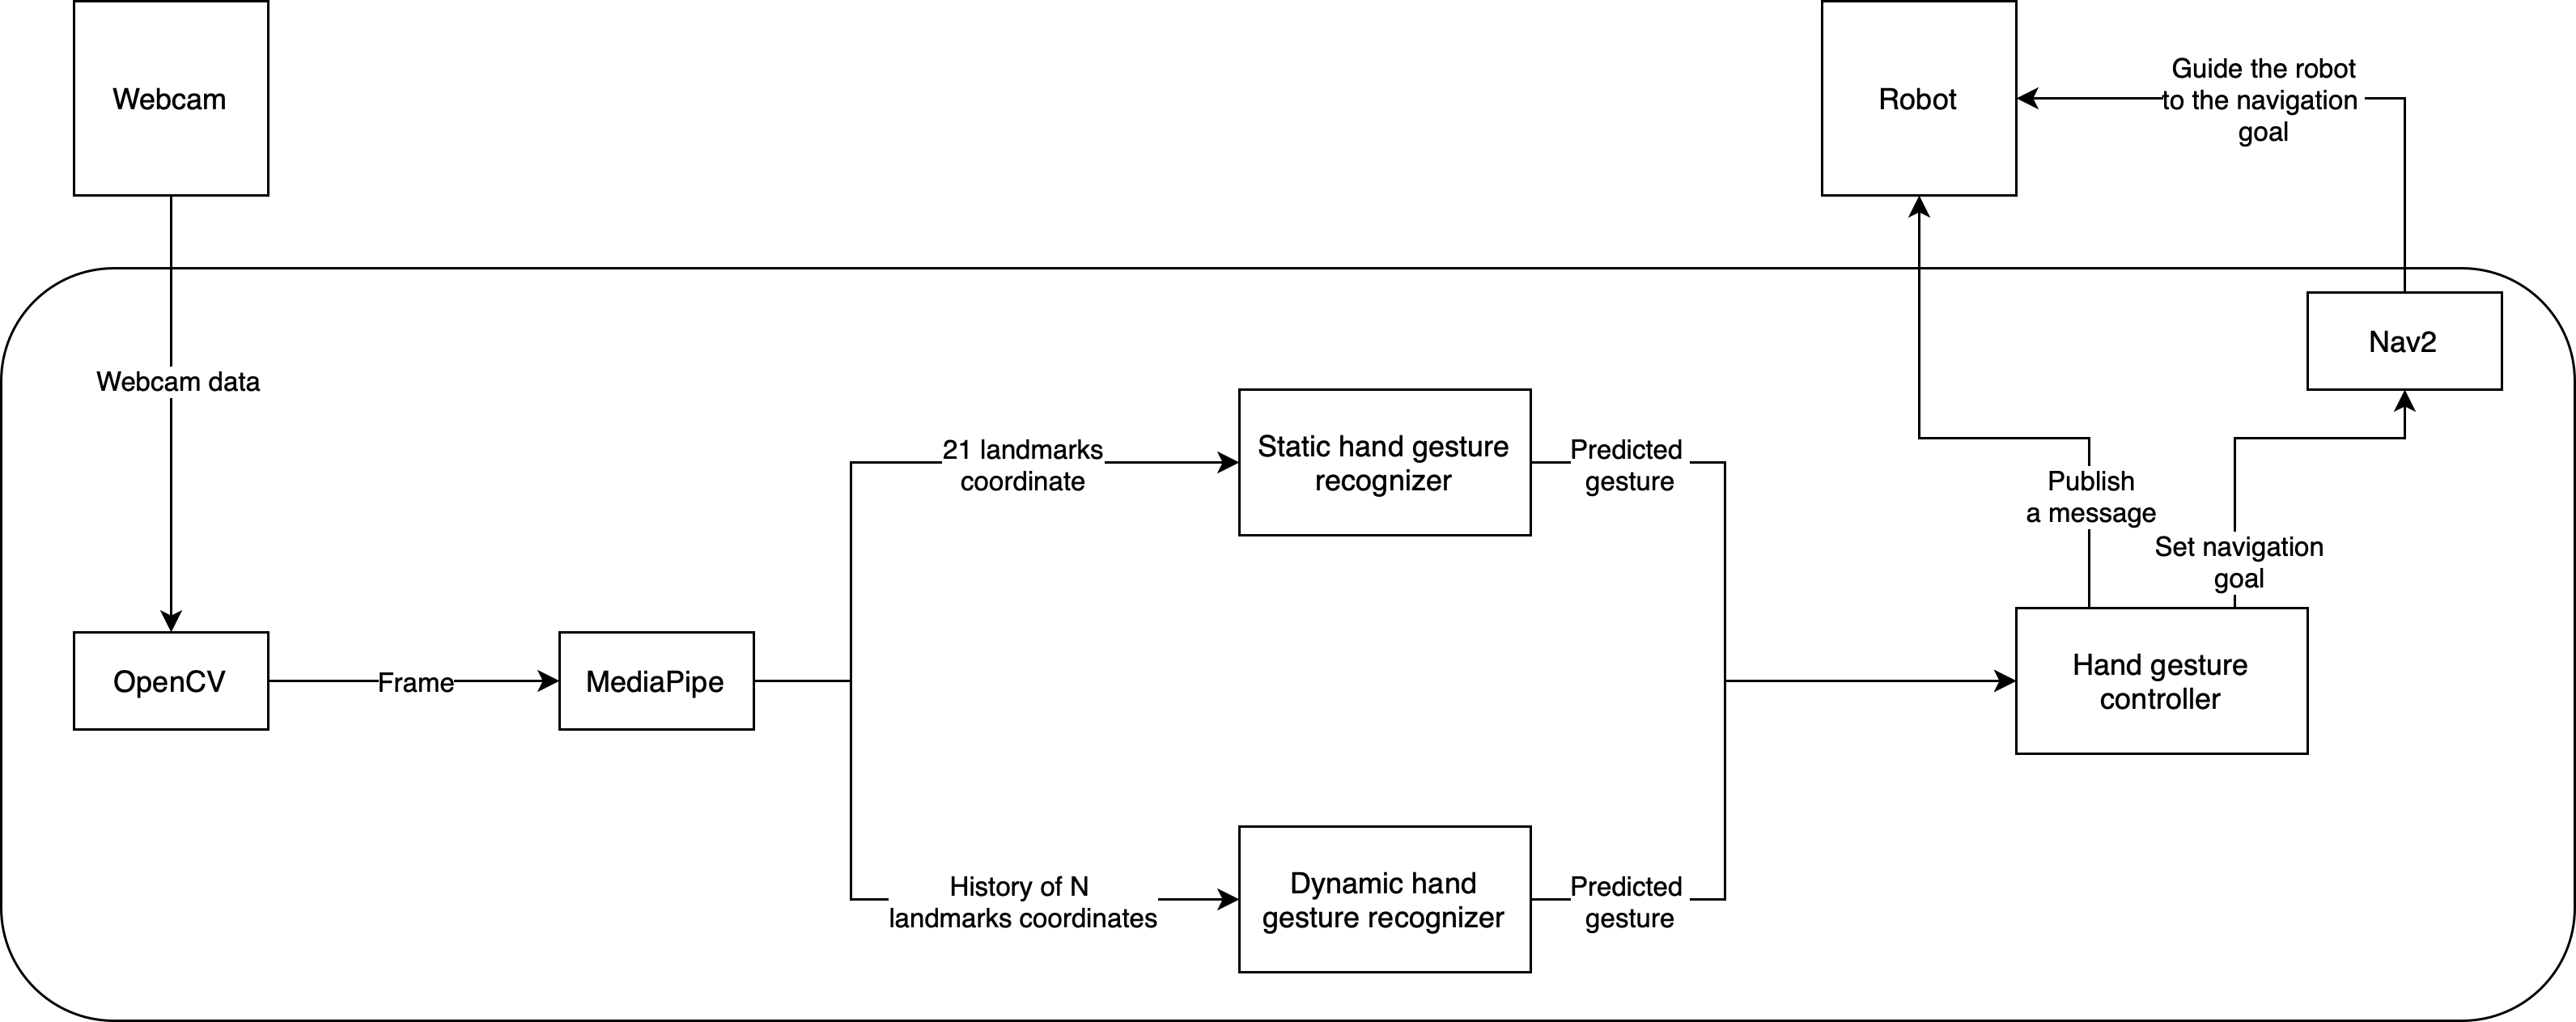
\includegraphics[width=\textwidth]{thesis/images/systemArchitectureOperational.png}
    \caption{Data flow in operational mode.}
    \label{fig:system_architecture_operational}
\end{figure}

Figure~\ref{fig:system_architecture_operational} shows the data flow in the operational mode:
\begin{enumerate}
    \item OpenCV receives the data from the webcam and converts it into a frame;
    \item the frame is given as input to MediaPipe, which handles the hand tracking task and returns the list of landmarks if a hand is detected in the frame;
    \item the landmarks in the frame are given as input to the ``static hand gesture recognizer'' model. Meanwhile, the landmarks in the frames along with those from the previous $N$ frames are given as input to the ``dynamic hand gesture recognizer'';
    \item both the recognizers return the predicted gesture;
    \item both the predicted gestures are taken into input by the ``hand gesture controller'' that decides which action to execute. Section~\ref{ss:hand_gesture_controller} describes in more detail how it works. Generally, it can publish a message on a \acrshort{ROS}' topic or set a navigation goal through the ``Nav2'' package.
\end{enumerate}

\subsubsection{Learning mode}
In this mode, users can choose to add a new gesture or enhance an already existing one by adding more data to the dataset. In both cases, a command-line interface is used to interact with the user and guide it through the process.
\begin{figure}[H]
    \centering
    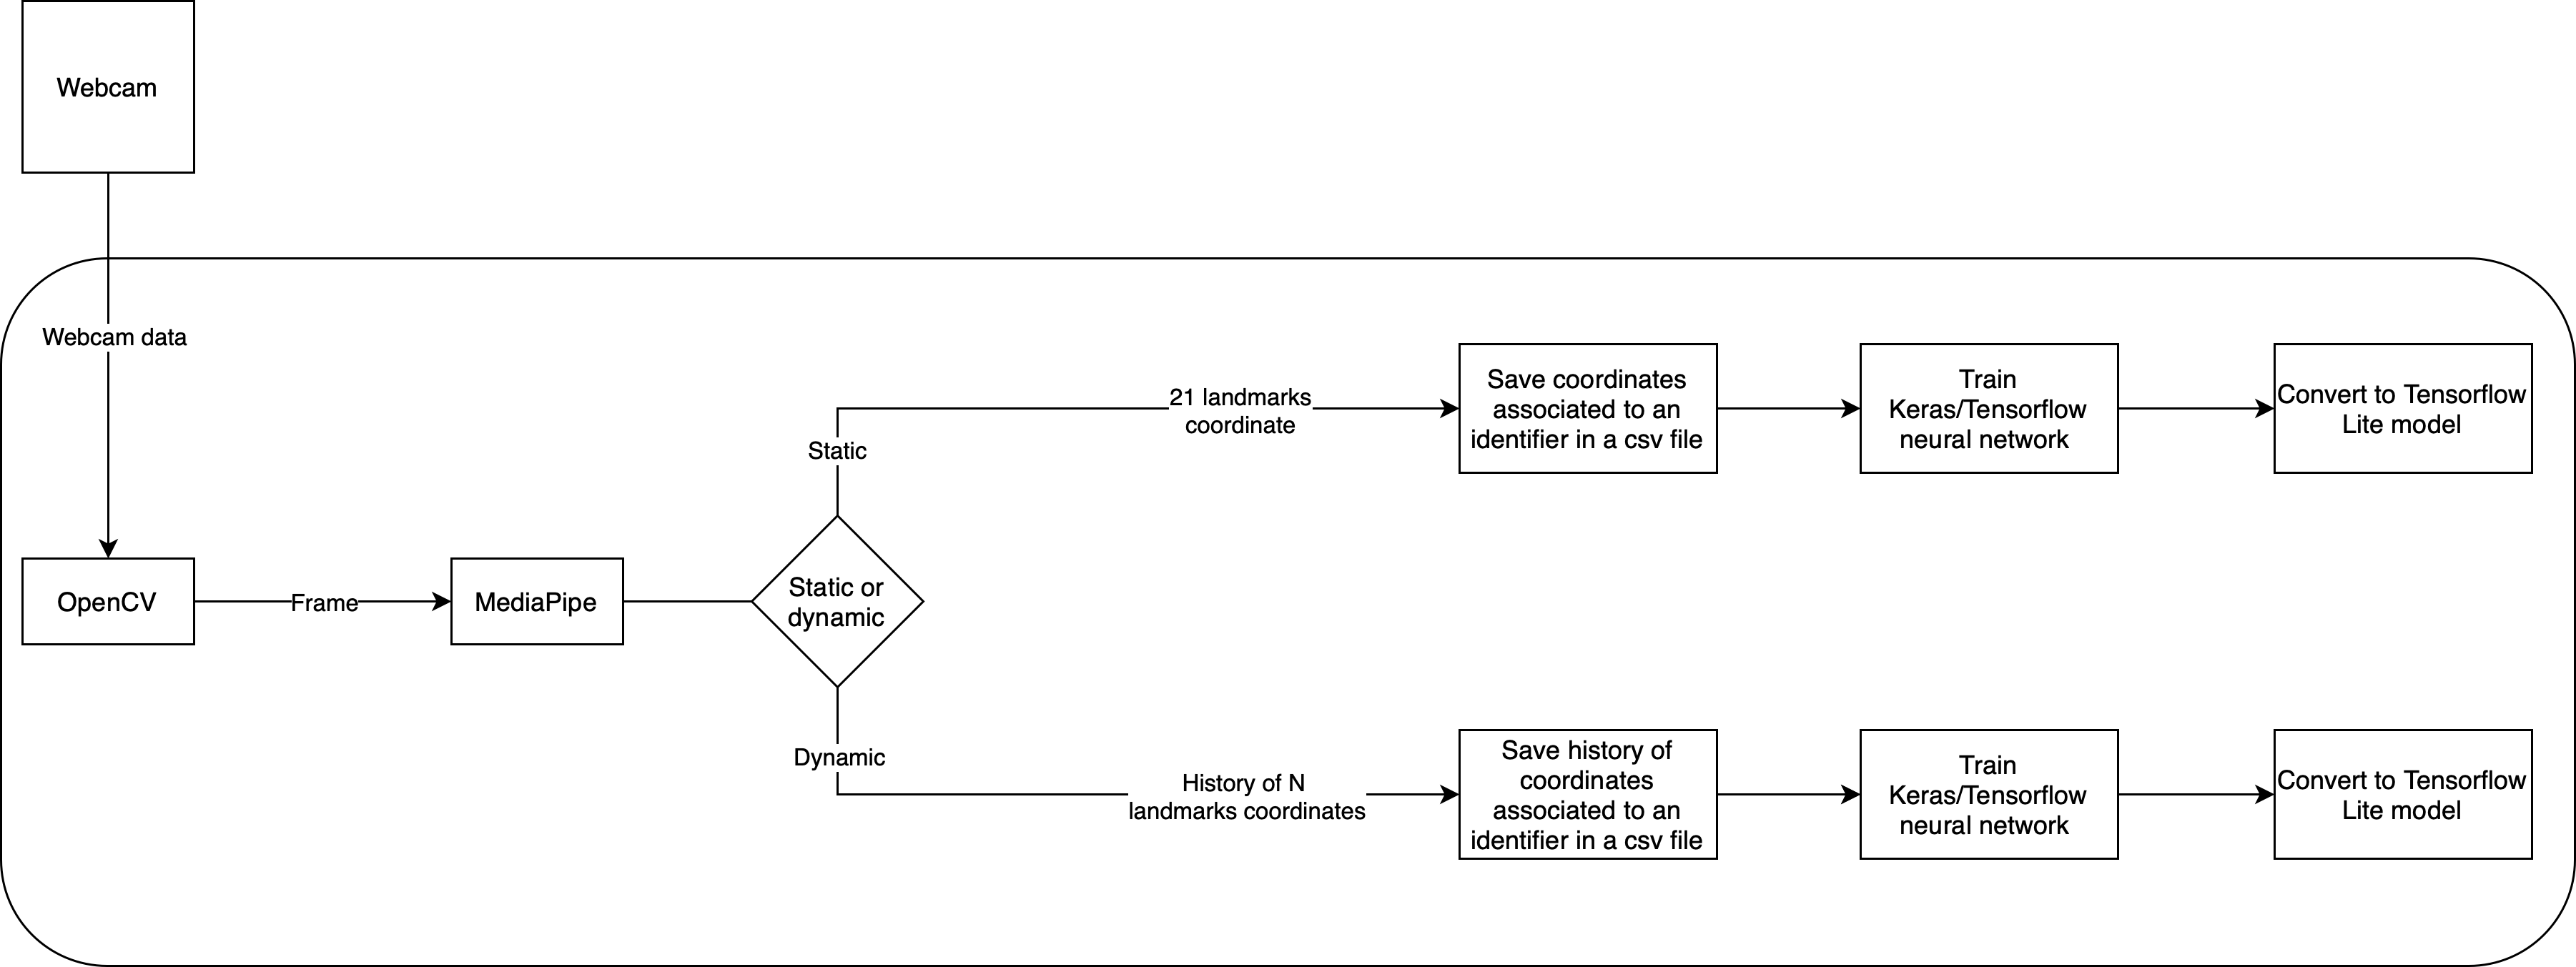
\includegraphics[width=\textwidth]{thesis/images/systemArchitectureTraining.png}
    \caption{Data flow in learning mode.}
    \label{fig:system_architecture_learning}
\end{figure}
Figure~\ref{fig:system_architecture_learning} shows the data flow in the learning mode:
\begin{enumerate}
    \item OpenCV receives the data from the webcam and converts it into a frame;
    \item the frame is given as input to MediaPipe, which handles the hand tracking task and returns the list of landmarks if a hand is detected in the frame;
    \item if users choose to add a new static gesture or enhance an existing one, the landmarks in the frame are saved in the CSV file with the identifier number that refers to the label of the gesture. Otherwise, if users choose to add a new dynamic gesture or enhance an existing one, the landmarks in the frames along with those from the previous $N$ frames are saved in the CSV file with the identifier number that refers to the label of the gesture.
    \item the associated neural network has been trained;
    \item the model is converted into a TFLite model, ready to be used by the recognizer.
\end{enumerate}

\subsubsection{Macro mode}
This mode is similar to the operational but, instead of sending the command in real-time to a robot, users can choose to save a sequence of gestures in a text file or ``execute'' a previously saved macro file, sending its content to a robot. 
\begin{figure}[H]
    \centering
    \begin{subfigure}[b]{\textwidth}
        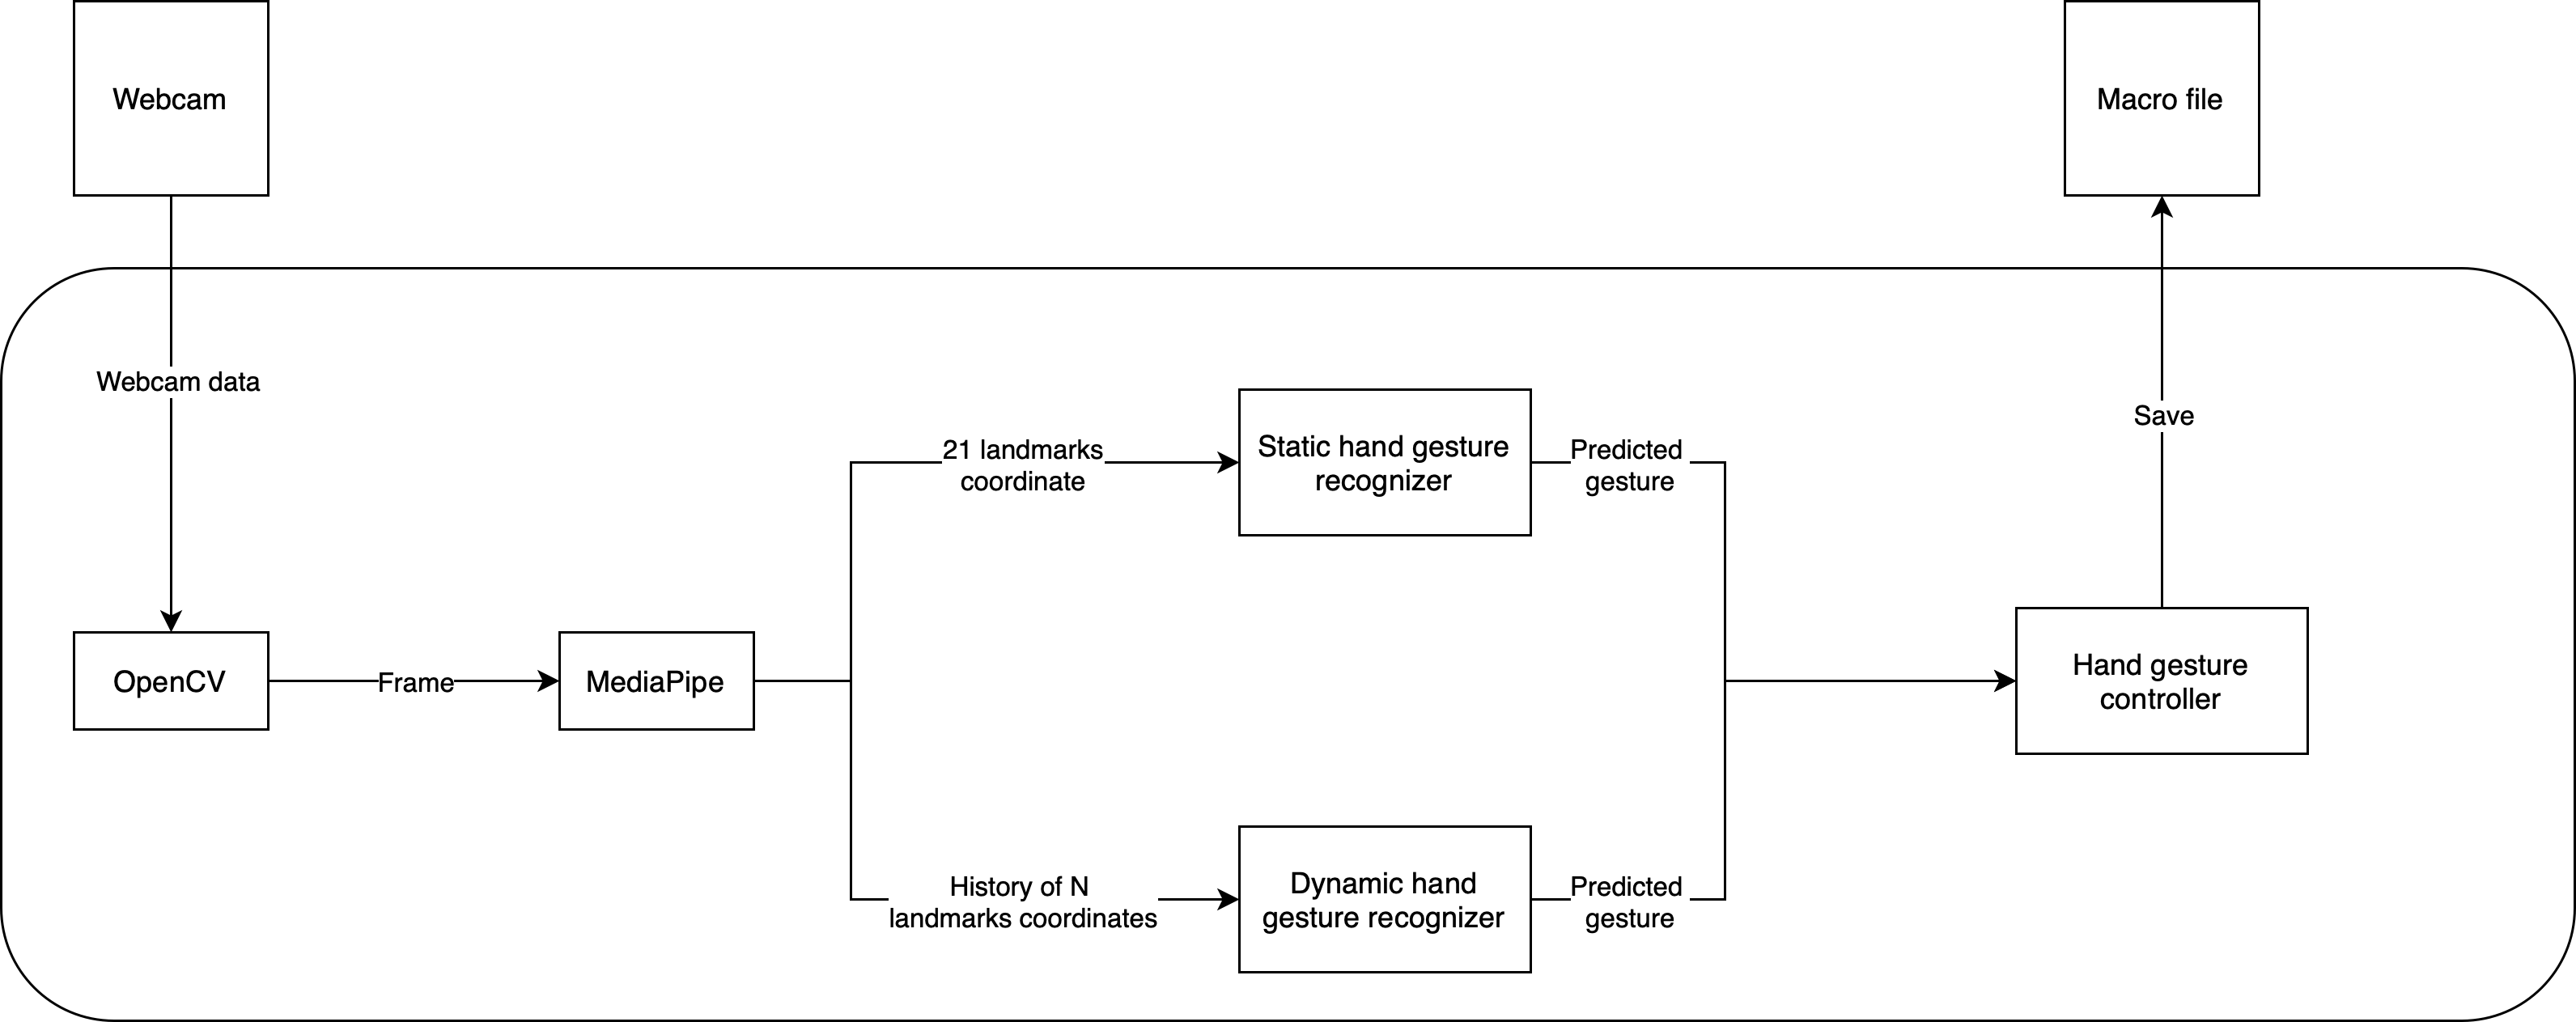
\includegraphics[width=\textwidth]{thesis/images/SystemArchitectureSaveMacro.png}
        \caption{Data flow when creating a new macro.}
        \label{fig:system_architecture_save_macro}
    \end{subfigure}
    \hfill
    \begin{subfigure}[b]{0.7\textwidth}
        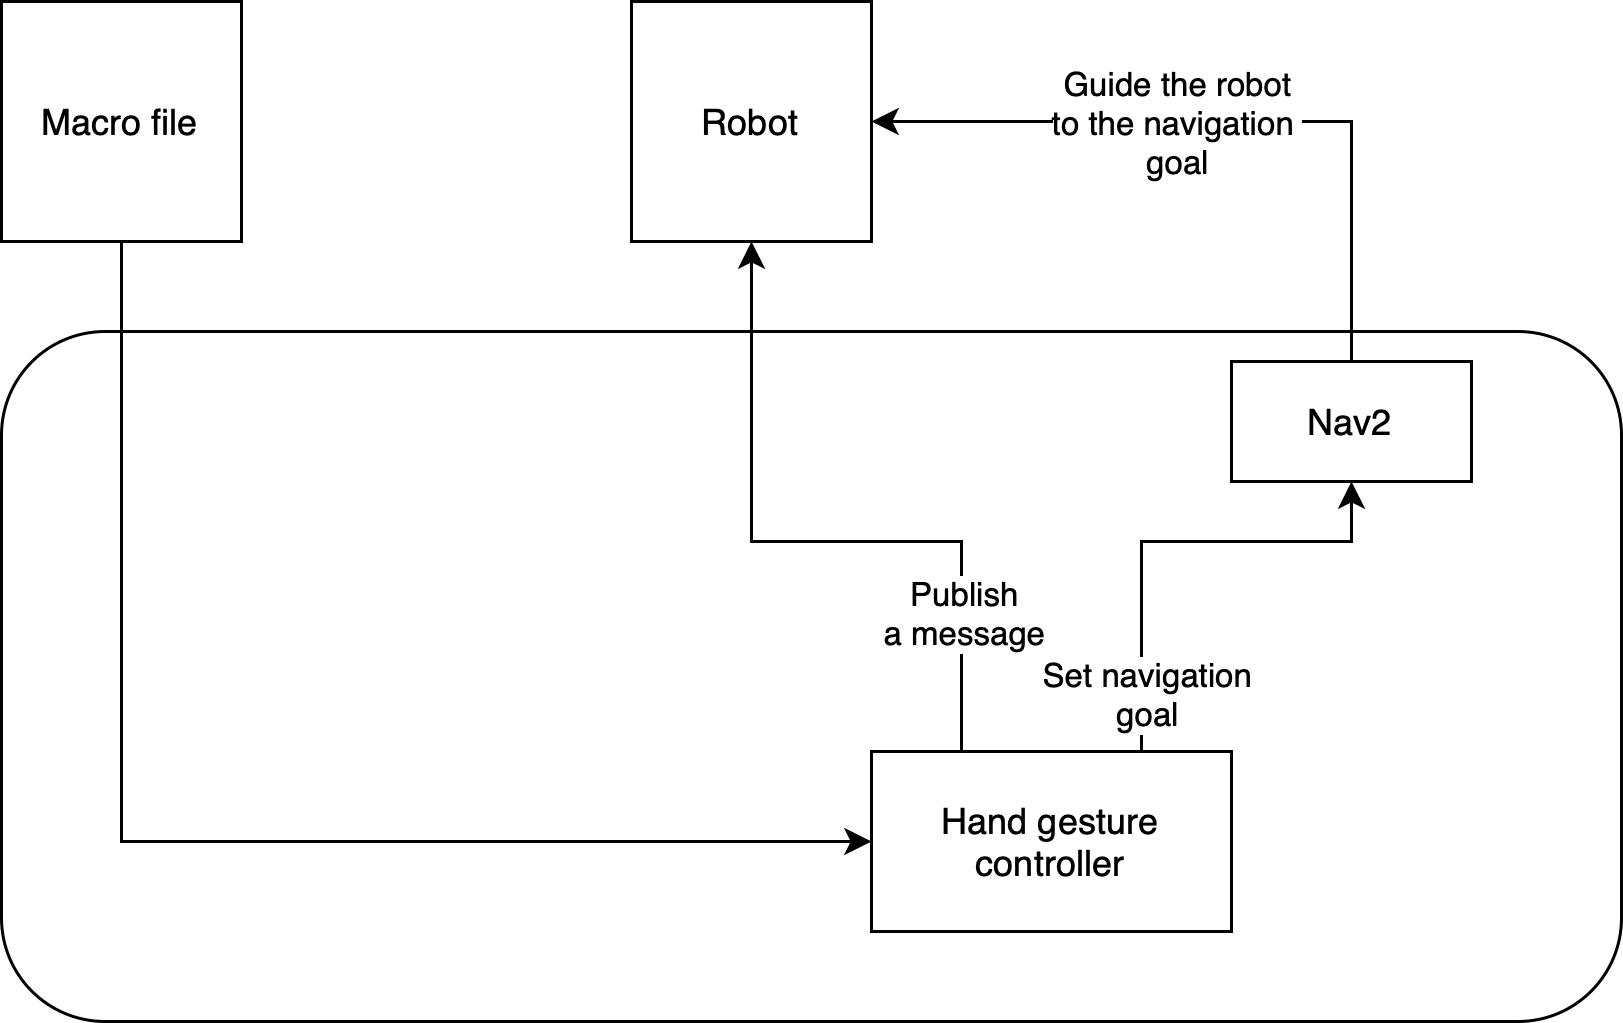
\includegraphics[width=\textwidth]{thesis/images/SystemArchitectureMacroRunner.png}
        \caption{Data flow when running a macro.}
        \label{fig:system_architecture_run_macro}
    \end{subfigure}
    
    \caption{Data flows in macro mode.}
    \label{fig:macro_data_flows}
\end{figure}
Figure~\ref{fig:system_architecture_save_macro} shows the data flow when users creates a new macro. The first part is the same as the operational mode explained in section~\ref{sss:operational_mode} but, instead of sending the command to the robot, it is saved in a text file. Figure~\ref{fig:system_architecture_run_macro} shows when a macro is run. The sequence of commands is read from the file created as described above. Then, the commands are given as input to the ``hand gesture controller'' which communicates with the robot as explained in section~\ref{sss:operational_mode}.

\subsection{Hand gesture recognizer}
The first challenge to solve was the design and implementation of the hand gesture recognizer. In particular, two types of hand gestures were considered: 
\begin{itemize}
    \item \textbf{static hand gestures}: in which the hand does not move and only a snapshot of the finger position is needed to recognize the gesture;
    \item \textbf{dynamic hand gesture}: in which the hand moves. In this case, a sequence of data is necessary to recognize the gesture. 
\end{itemize}
This diversity leads to two different neural networks to classify the hand gestures users are making. 

\subsubsection{Static hand gestures}
As reference, the set of static hand gestures chosen is the \gls{ASL} (in figure~\ref{fig:asl}). \textit{J} \textit{Z} are excluded because they involve a movement. To discriminate between dynamic and static gestures, I decided to prioritize the dynamic ones because users have to perform an action to activate them. Instead, with the static gestures, the hand does not move, and the recognizer will always return a possible prediction. Also, the numbers have been excluded. 

\begin{figure}
    \centering
    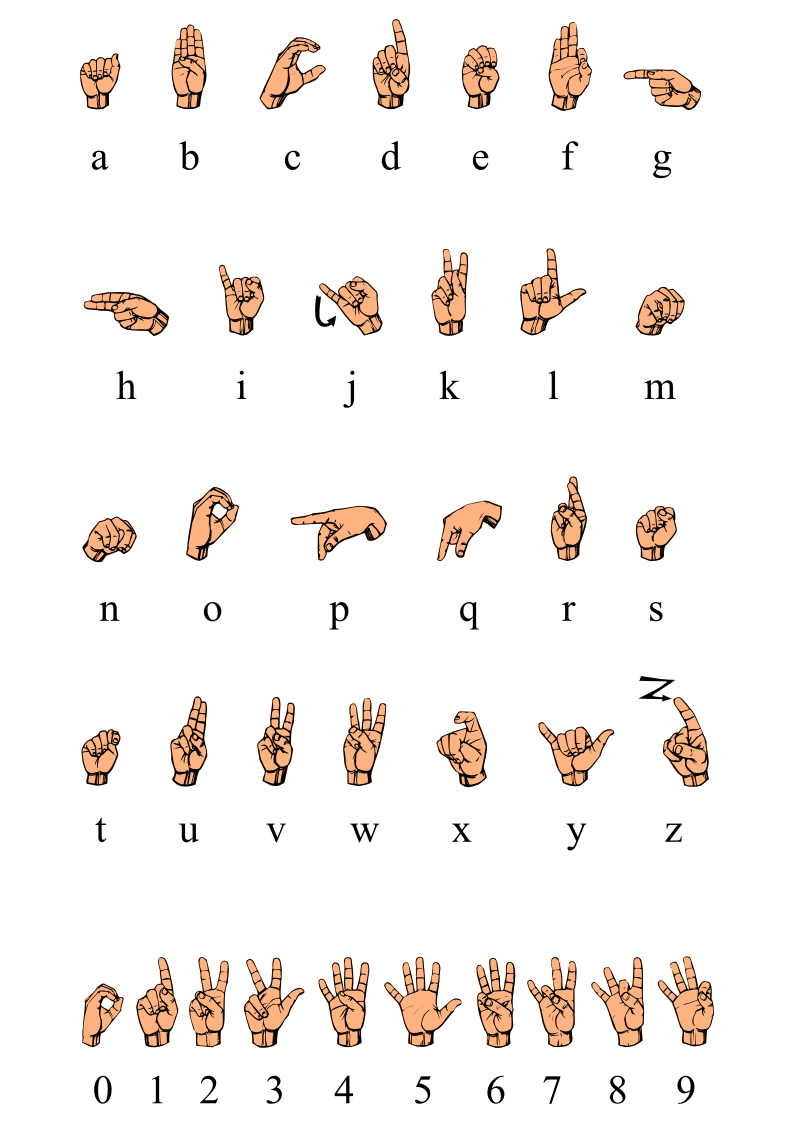
\includegraphics[width=0.8\textwidth]{thesis/images/asl.png}
    \caption{\glsdesc{ASL}~\parencite{img:asl}}\label{fig:asl}
\end{figure}

\paragraph{MediaPipe data}
From MediaPipe, the static hand gesture recognizer gets twenty-one landmarks per frame. These landmarks are shown in figure~\ref{fig:landmarksMediapipe}. The dataset is a CSV file where each line contains:
\begin{itemize}
    \item the identifier of the static hand gesture. It refers to the line in the label’s file; 
    \item 42 coordinates (i.e. X and Y) of the 21 landmarks, they are relative to the zeroth landmark (i.e. the wrist) and normalized. 
\end{itemize}

\paragraph{Deep neural network}\label{p:static_hand_gesture_deep_neural_network}
The neural network to recognize the hand gesture starting from MediaPipe's landmarks is a feed-forward network.
\begin{figure}[H]
    \centering
    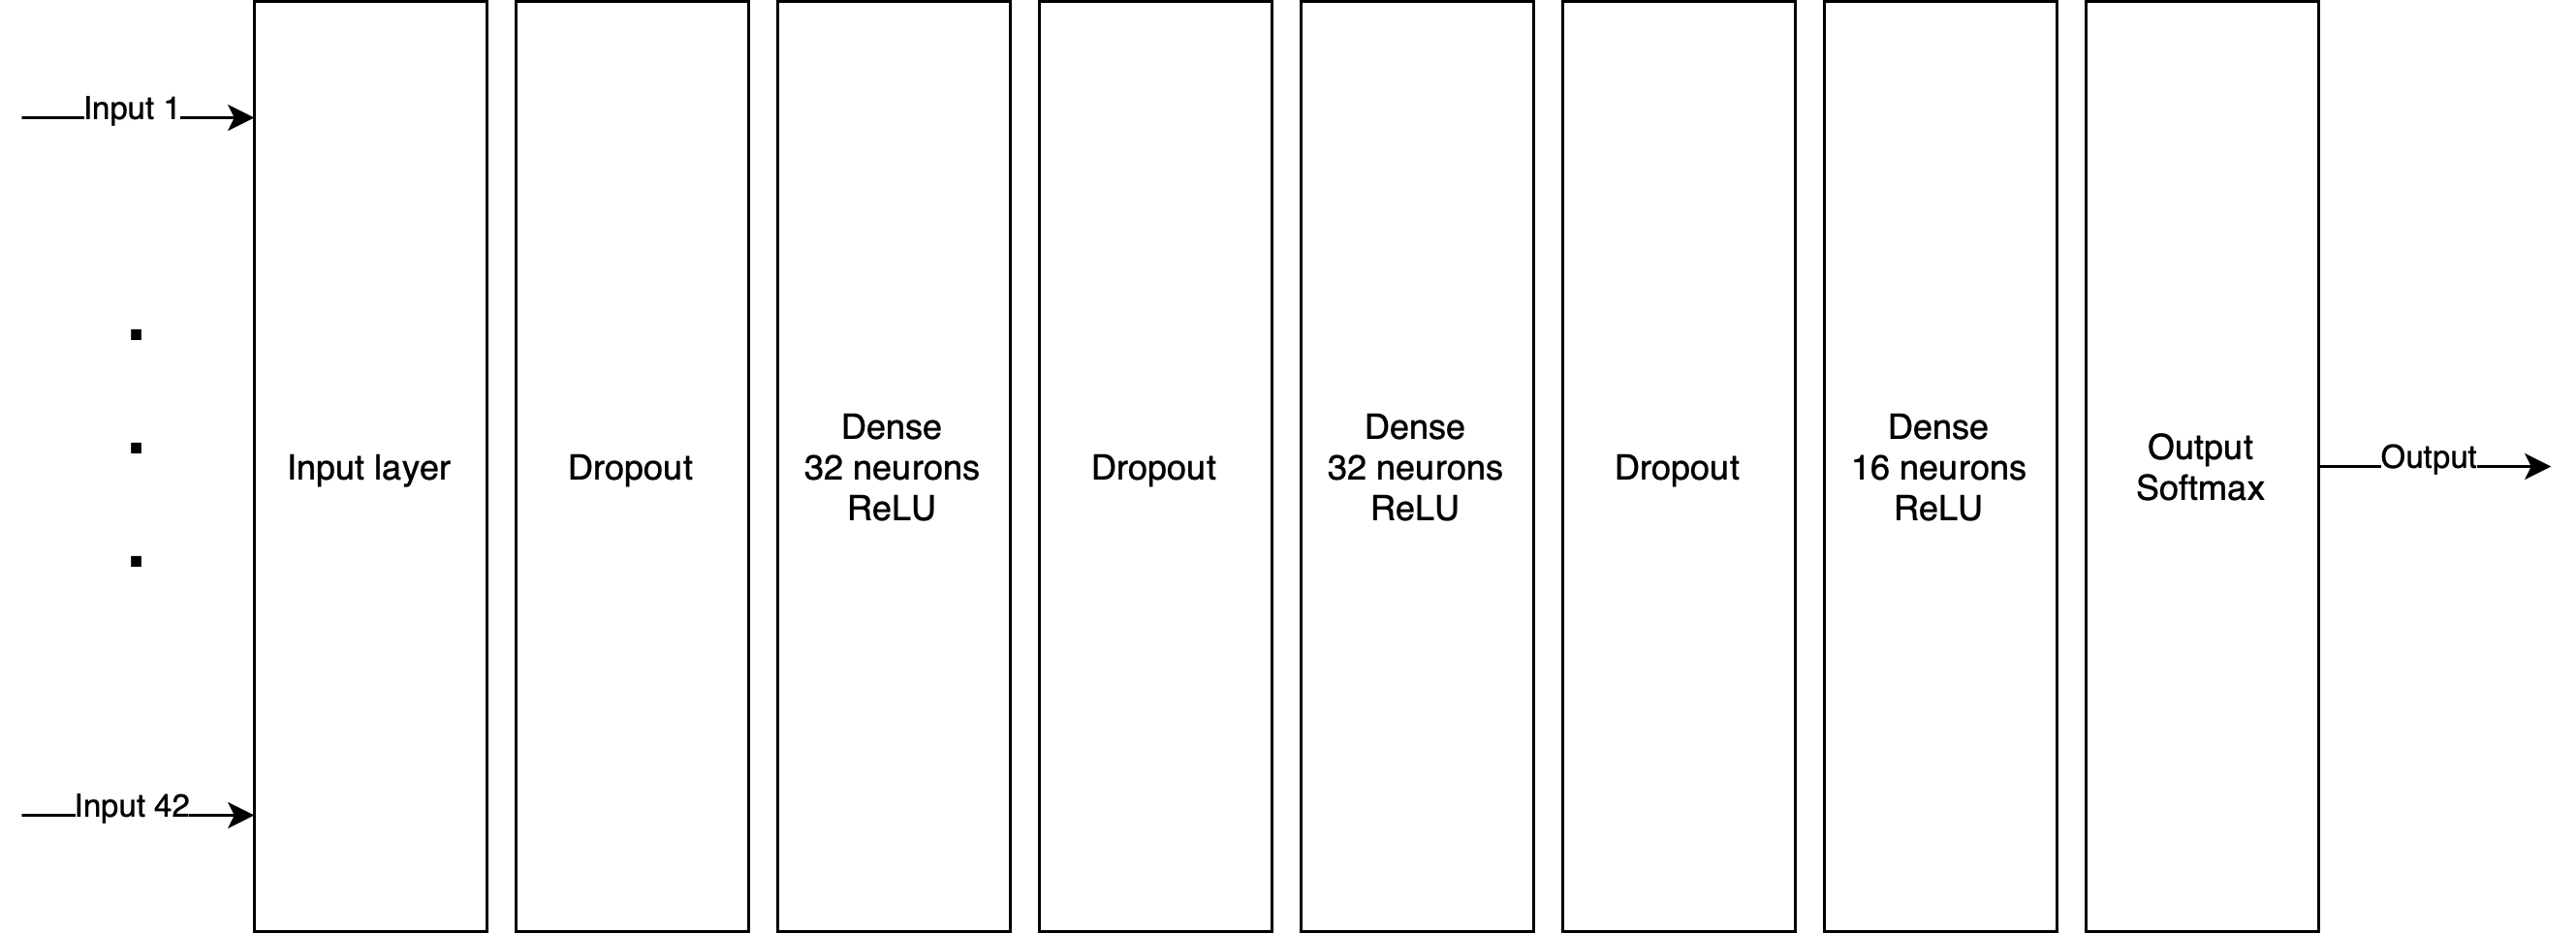
\includegraphics[width=\textwidth]{thesis/images/StaticHandGestureModel.png}
    \caption{Deep neural network for static hand gestures.}
    \label{fig:static_hand_gesture_model}
\end{figure}
Figure~\ref{fig:static_hand_gesture_model} presents the layers in the network:
\begin{itemize}
    \item \textbf{input layer}: it takes in input the data from the dataset. Exactly 42 float numbers, representing the relative and already normalized coordinates of the landmarks; 
    \item \textbf{dropout layer}: it randomly drops the input received, which helps prevent overfitting. If the input is kept, it is passed to the next layer unchanged; 
    \item \textbf{dense layer}: it is a layer composed of N neurons. Every one of them takes every input received from the previous layer and uses the ReLU activation function to return the output;
    \item \textbf{output layer}: it is a dense layer with the softmax as activation function.
\end{itemize}

\paragraph{Training}\label{p:static_hand_gesture_training}
To train the network the script:
\begin{enumerate}
    \item reads the dataset file;
    \item if users request it, a random under-sampling is applied;
    \item divides the dataset into three non-overlapping subsets (train set, validation set, and evaluation set);
    \item builds and compiles the network with callbacks to save the model during training, to early stop the training if the loss function does not improve anymore, and log analytics for Tensorboard; 
    \item trains the network on the train set and validates it with the validation set, gathering accuracy, loss function value, and time spent;
    \item evaluates the network on the evaluation set;
    \item converts the model to a Tensorflow Lite model.
\end{enumerate}

\subsubsection{Dynamic hand gestures}
Six dynamic hand gestures have been chosen to test the system:
\begin{itemize}
    \item \textbf{Z}: taken from the \acrshort{ASL};
    \item \textbf{J}: taken from the \acrshort{ASL};
    \item \textbf{go to}: to communicate to the robot to move to a location;
    \item \textbf{pick up}: to communicate to the robot to pick up a parcel;
    \item \textbf{drop down}: to communicate with the robot in order for the parcel to be dropped down;
    \item \textbf{static}: for when the hand is not moving.
\end{itemize}
The recognition of the dynamic hand gestures, except for \textit{static}, is prioritized over static ones.
\paragraph{MediaPipe data}
From MediaPipe, the dynamic hand gesture recognizer gets $N \times history\_length$ landmarks coordinates per each frame. Where $N$ is the number of landmarks, shown in figure~\ref{fig:landmarksMediapipe}, saved, and $history\_length$ is the previous frames from which to take the landmarks. Indeed, users can choose how many landmarks to save and how many previous frames to consider. This data is saved in a CSV file where each line contains: 
\begin{itemize}
    \item the identifier of the dynamic hand gesture. It refers to the line in the label’s file; 
    \item $N \times history\_length$ coordinates relatives to the zeroth landmark (i.e. the wrist) and normalized.
\end{itemize}

\paragraph{Deep neural network}
I tried two neural networks to recognize the dynamic hand gestures starting from MediaPipe's landmarks history. The first one is a feed-forward network.
\begin{figure}[H]
    \centering
    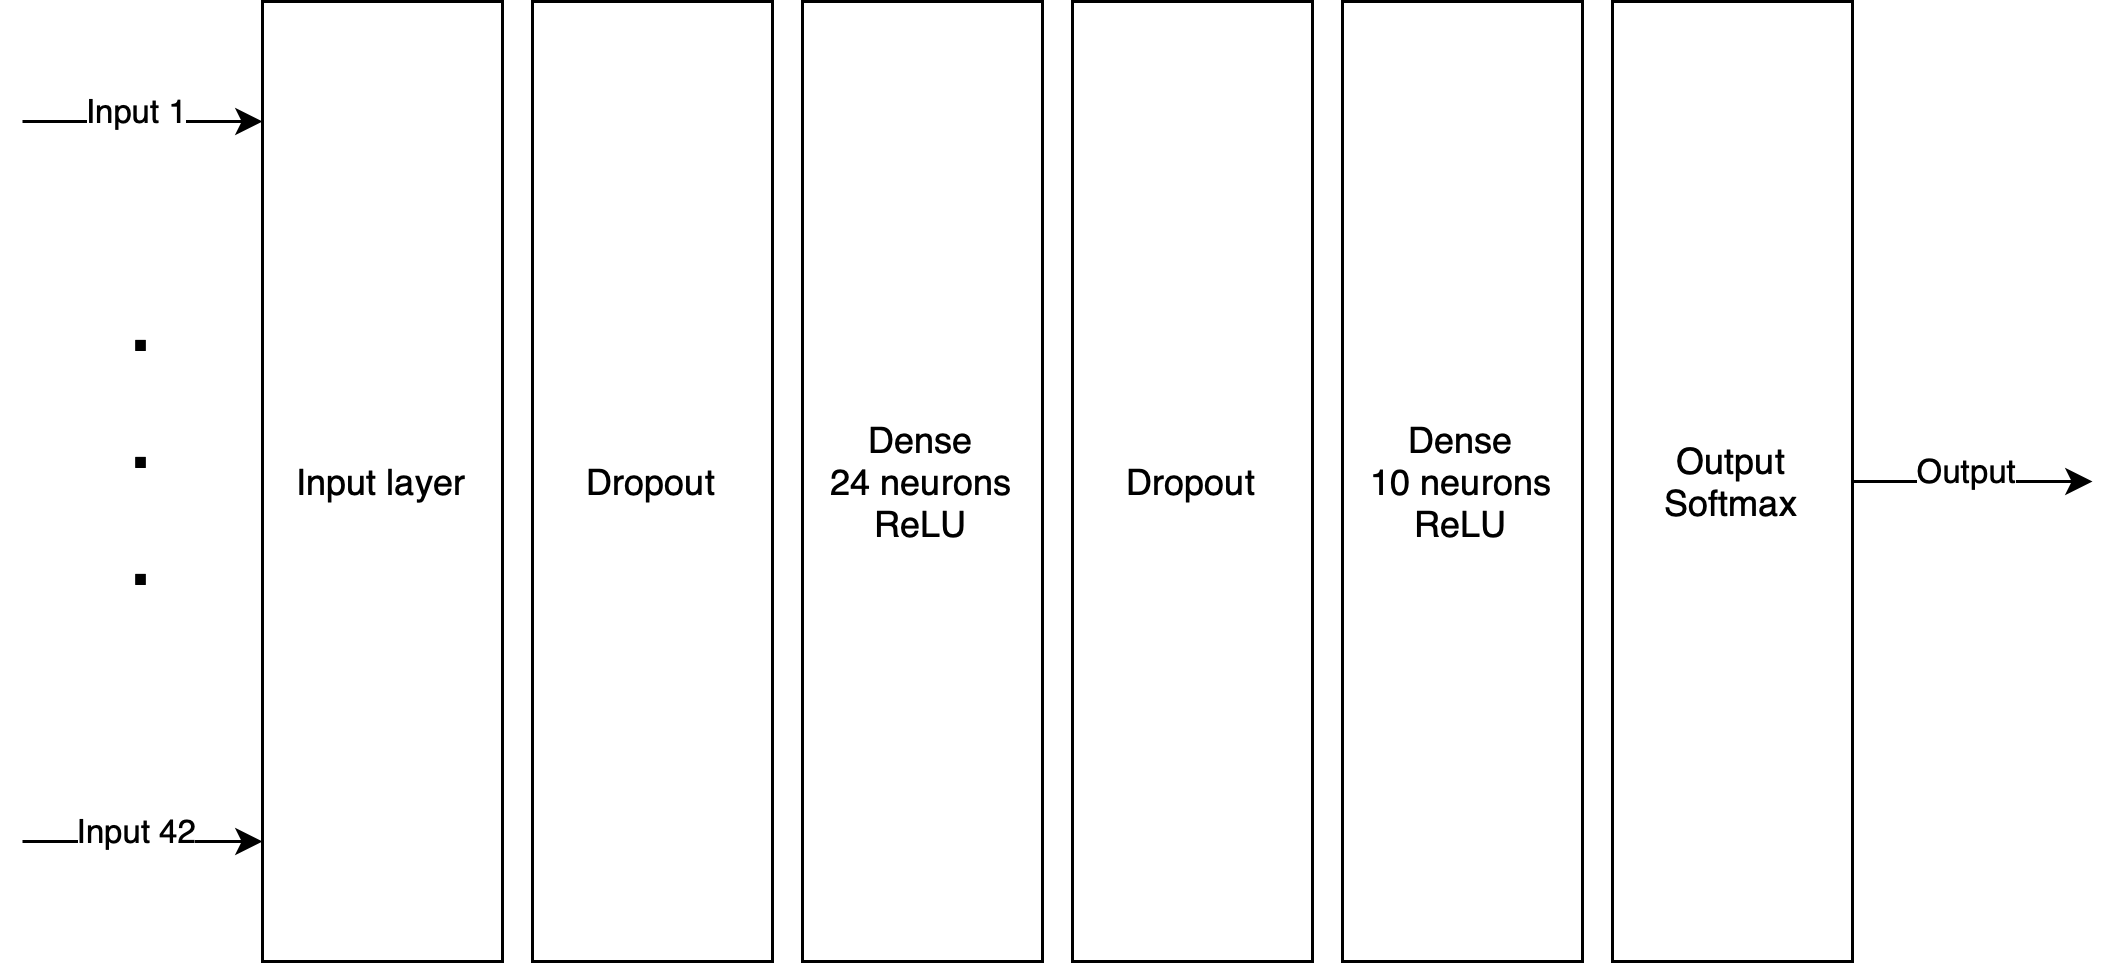
\includegraphics[width=\textwidth]{thesis/images/DynamicHandGestureModelFeedForward.png}
    \caption{Deep feed-forward neural network for dynamic hand gestures.}
    \label{fig:ff_model_dynamic_hand_gestures}
\end{figure}
Figure~\ref{fig:ff_model_dynamic_hand_gestures} presents the layers in the network.  They are the same as those present in paragraph~\ref{p:static_hand_gesture_deep_neural_network}.
The second one is an \acrshort{LSTM} network.
\begin{figure}[H]
    \centering
    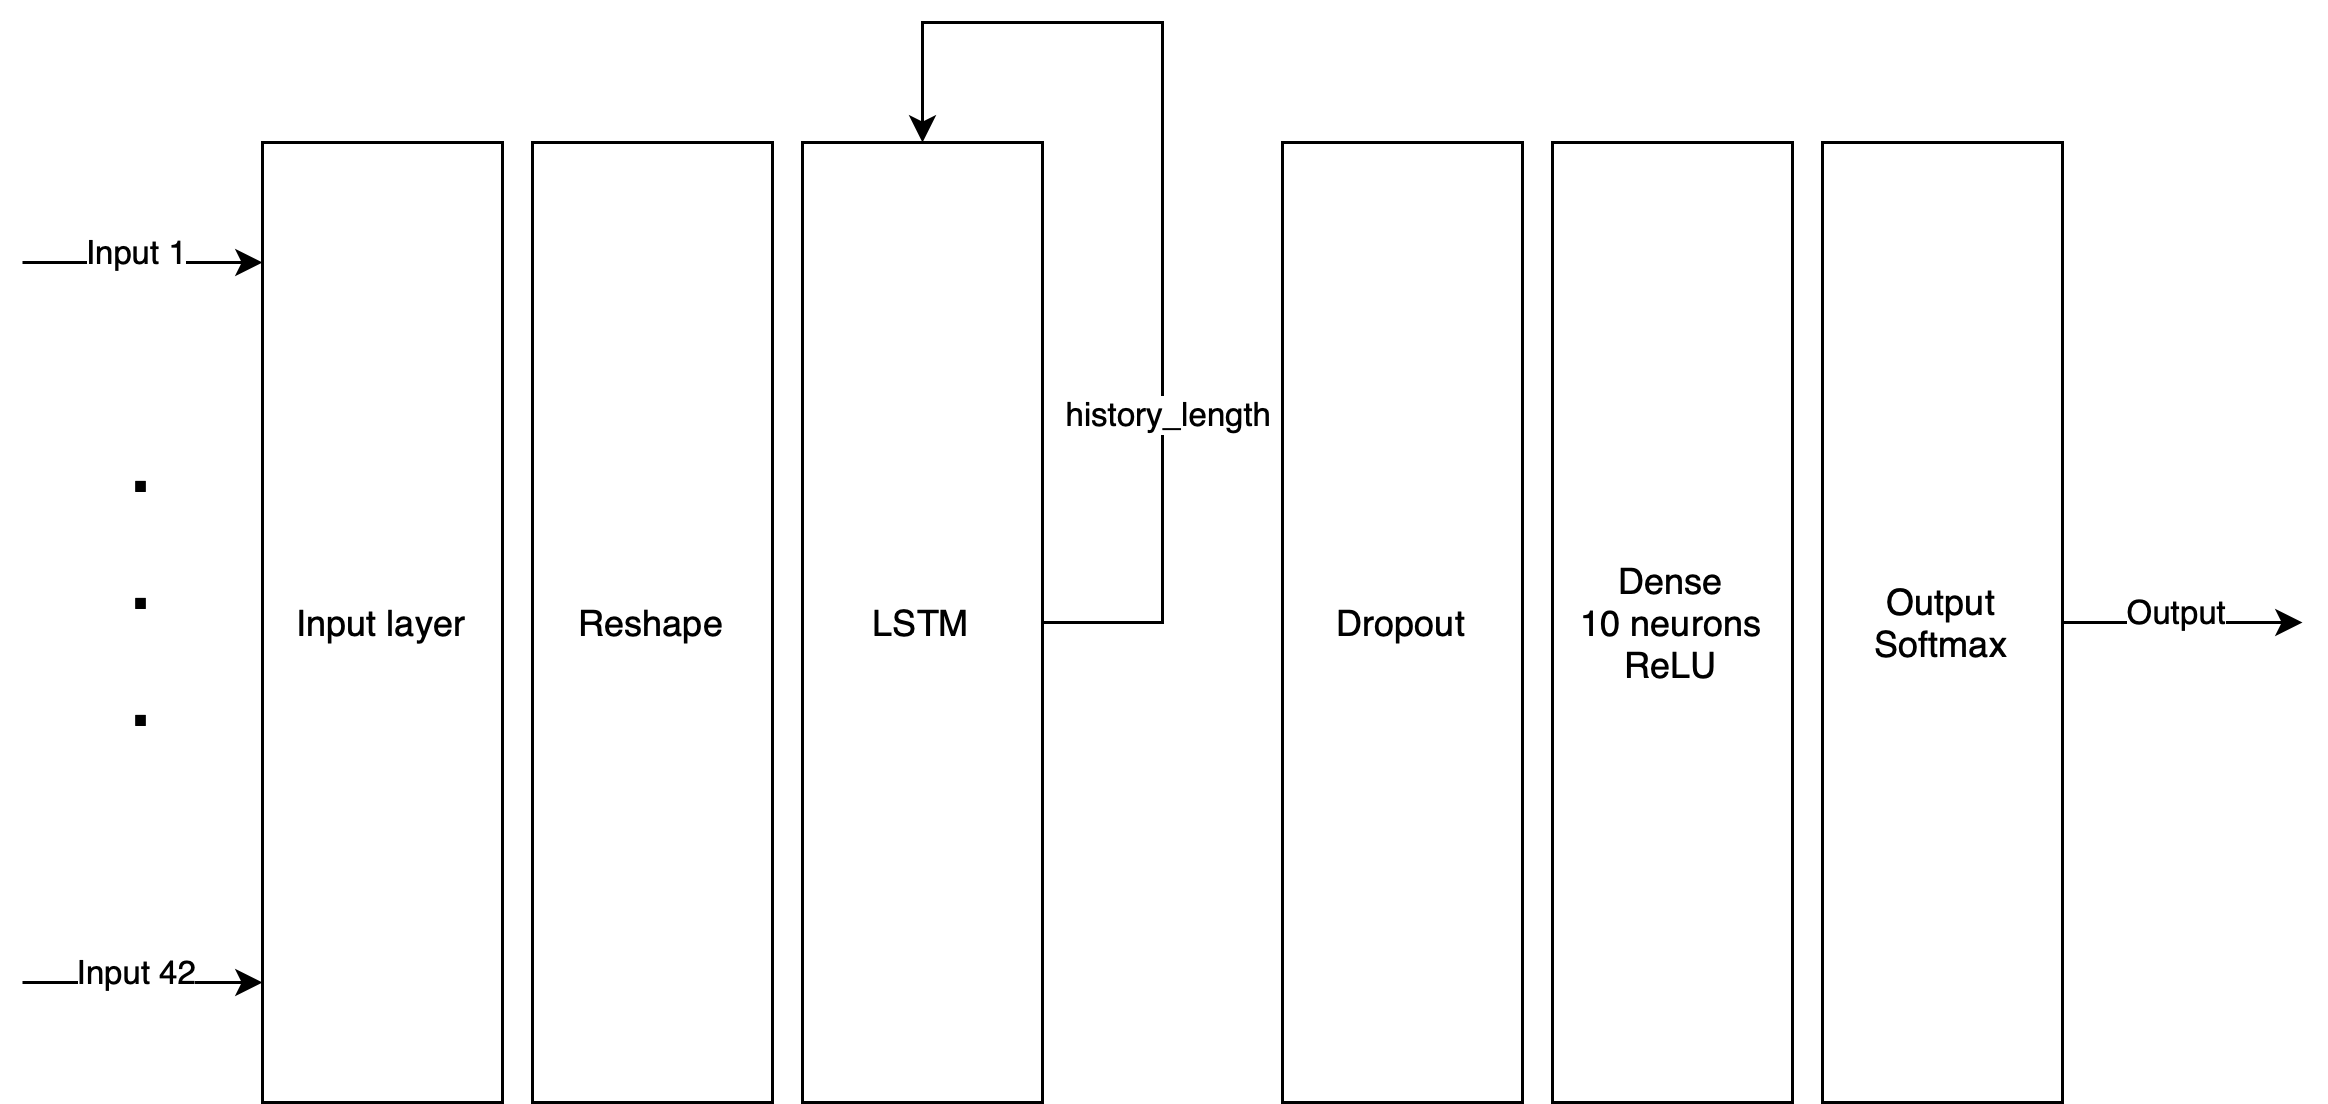
\includegraphics[width=\textwidth]{thesis/images/DynamicHandGestureModelLSTM.png}
    \caption{\acrshort{LSTM} neural network for dynamic hand gestures.}
    \label{fig:lstm_model_dynamic_hand_gestures}
\end{figure}
In the model presented in figure~\ref{fig:lstm_model_dynamic_hand_gestures}, the input is first reshaped to group together the landmark coordinates from the same frame. Then an LSTM layer is used, cycling through the  $history\_length$. This model should perform better because it exploits the potential of a recurrent neural network to learn from a time series.

\paragraph{Training}
The training is similar to the one presented in paragraph~\ref{p:static_hand_gesture_training}, with the addition of the possibility for the users to choose which model to use.

\subsubsection{Early stopping}
Early stopping is the method adopted to specify an arbitrarily high number of epochs. With this technique, the end of the training is triggered by the recorded variation of a specified metric. In other words, when a metric does not change (or changes just a little) for a specified number of epochs, then the training can be considered ended.\\

This technique has been used in both static hand gesture training and dynamic hand gesture training. The metric monitored was the loss on the validation dataset, and the number of epochs to control was fifty.

\subsection{Hand gesture controller}\label{ss:hand_gesture_controller}
The hand gesture controller is the component that takes as input the recognized hand gestures and converts them into the correct command for the robot. To better have a modular system the hierarchy in figure~\ref{fig:controller-class-diagram} has been implemented.

\begin{figure}[H]
    \centering
    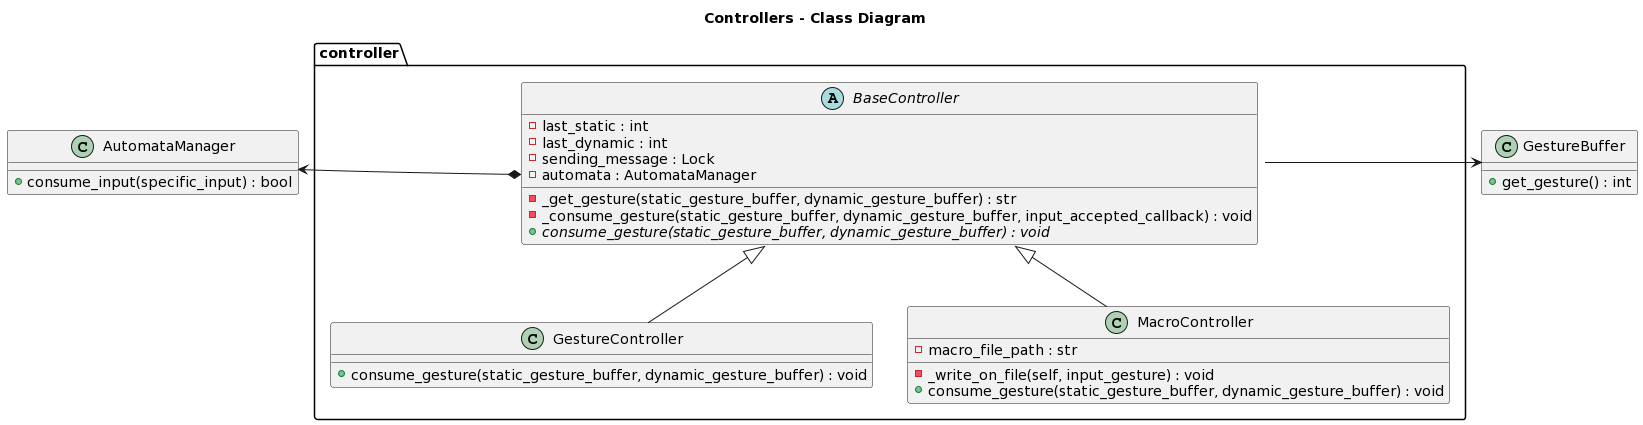
\includegraphics[width=1\textwidth]{thesis/images/ControllerClassDiagram.png}
    \caption{UML class diagram for the hand gesture controller.}
    \label{fig:controller-class-diagram}
\end{figure}

The class \textit{BaseController} handles the communication between the hand gesture recognizer and the automaton that will communicate with the robot. The \textit{HandGestureController} implements the method \textit{consumer\_input} telling to the automaton to send the messages to the robot in contrast to the \textit{MacroController} that does not. Instead, the \textit{MacroController} saves on a text file the sequence of gestures made by the operators with the purpose to use them in another moment.

\subsubsection{Automaton}\label{sss:automaton_methodology}
To ensure the correctness of the sequence of gestures, users have to describe it as a finite-state automaton. The configuration file is a JSON file that requires the users to define:
\begin{itemize}
    \item the initial state;
    \item a list of transitions. Each transition is defined by:
    \begin{itemize}
        \item from which state it comes;
        \item to which state it is directed;
        \item with which element of the alphabet ($\Sigma$) it is triggered;
        \item the action to perform when the transition is triggered. It can be:
        \begin{itemize}
            \item \textbf{null} when no action is performed;
            \item \textbf{set a navigation goal} specifying the coordinates;
            \item \textbf{send a message} specifying on which topic publish the message, its type, and the raw data to send.
        \end{itemize}
    \end{itemize}
\end{itemize}
To better interact with the robot, the coordinates and the raw data for the messages can be interpolated with the element of the alphabet that trigger the transition. An example of configuration file can be found in~\ref{appendix:automaton_configuration_file}.\\

Four seconds elapse between the input of two commands, if the first one does not involve any action. Otherwise, before to accept another input the controller waits for the action to end. This is made to allow the users to change the gesture they are doing. The amount of time is configurable but four seconds have been shown to be sufficient.\\

There is not a common way to evaluate how much complex and understandable a JSON file is but, since it is a file that has to be written and read by an user, it is important to give an evaluation of it. The method adopted to calculate the complexity considers the depth and the type of fields per object: 
\begin{itemize}
    \item strings, numbers, and null values have a complexity of $1$;
    \item arrays have a complexity equal to $1 + (average\, complexity\, of\, nested\, elements)$;
    \item objects have complexity equal to the complexity of their elements;
    \item every nested elements have a weight $d$ that multiplies the complexity score. 
\end{itemize}
The algorithm to compute the complexity has been implemented in JavaScript and it is showed in~\ref{appendix:complexity_algorithm}. 

\subsection{Integration with ROS}
The integration with \acrshort{ROS} is managed through two Python packages:
\begin{itemize}
    \item \textbf{rclpy}: it comes with the installation of \acrshort{ROS} as described in the documentation and it handles the raw communication between the hand gesture controller and the robot;
    \item \textbf{nav2}: package which implement the Nav2 navigation algorithm. It has been installed with pip after cloning the GitHub repository\footnote{\href{https://github.com/ros-planning/navigation2.git}{https://github.com/ros-planning/navigation2.git}} with the following command:\newline\texttt{pip3 install navigation2/nav2\_simple\_commander/}
\end{itemize}
First and foremost the \textit{rclpy} is initialized with the statement \texttt{rclpy.init()}. Then, the hand gesture controller can either publish a message to a topic or set a goal for navigation based on the triggered automaton transition.
\begin{itemize}
    \item send a message: the topic, the message type, and the data for the message are taken from the transition details described in the automaton configuration file. Then, the correct publisher is retrieved and used to publish the message. This kind of action exploits the message exchange system of topics explained in section~\ref{p:exchange_message_with_topics};
    \item set a navigation goal: the coordinates are taken from the transition details described in the automaton configuration file. Then, the position is given as input to the navigator which returns a feedback until the task is completed. When the task is completed, it return the status of the operation:
    \begin{itemize}
        \item succeeded: if the robot reach the goal correctly;
        \item cancelled: if the operators cancelled the task;
        \item failed: if the robot can't reach the set goal for any reason.
    \end{itemize}
\end{itemize}

\subsection{User interface}
A command line interface is the first interface with which users interact. It asks a few questions about what users wants to do. They can answer writing on the terminal. It is designed to guide users in the execution of the possible tasks:
\begin{itemize}
    \item launch the operation mode;
    \item launch the learning mode asking which dataset is to be edited and other gesture's data;
    \item launch the macro mode asking if users want to execute an existing macro or to create a new one.
\end{itemize}
Figure~\ref{fig:activity_diagram_cli} show the complete flaw chart with all the possibilities for the users.
\begin{figure}[H]
    \centering
    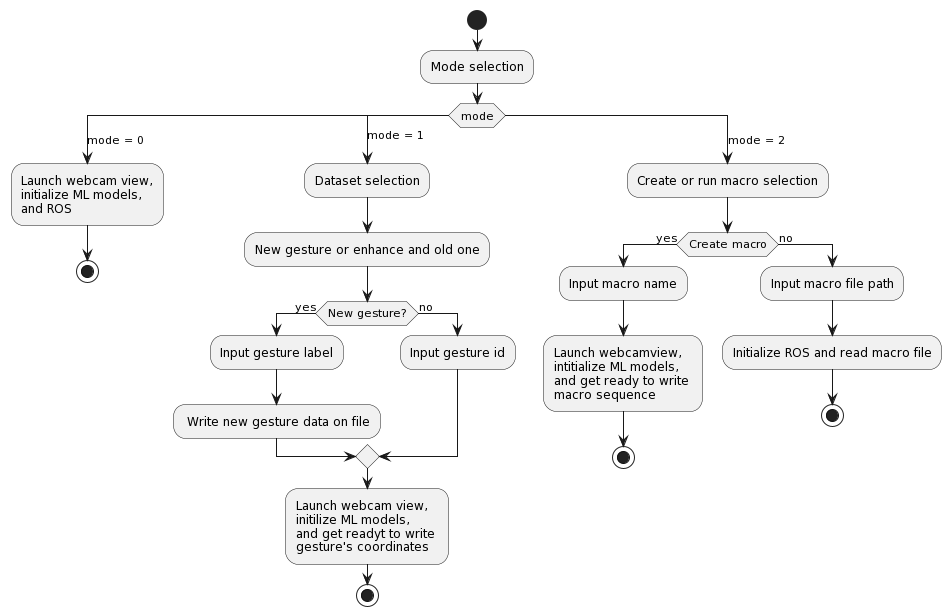
\includegraphics[width=\textwidth]{thesis/images/activity_diagram_cli.png}
    \caption{Activity diagram of the command line interface}
    \label{fig:activity_diagram_cli}
\end{figure}

When users select a mode that involves the use of the camera a window appears showing to them what the camera is watching, the number of FPS, the recognized gestures, and the selected mode. Moreover, it shows also the hand's landmarks (i.e. the black points), the joints between them, and the landmarks used for the history of key-points in green with a trail when the hand moves. Figure~\ref{fig:example_ui}, for example, shows the recognition of the gesture \textit{F} as static gesture and \textit{Static} as dynamic.

\begin{figure}
    \centering
    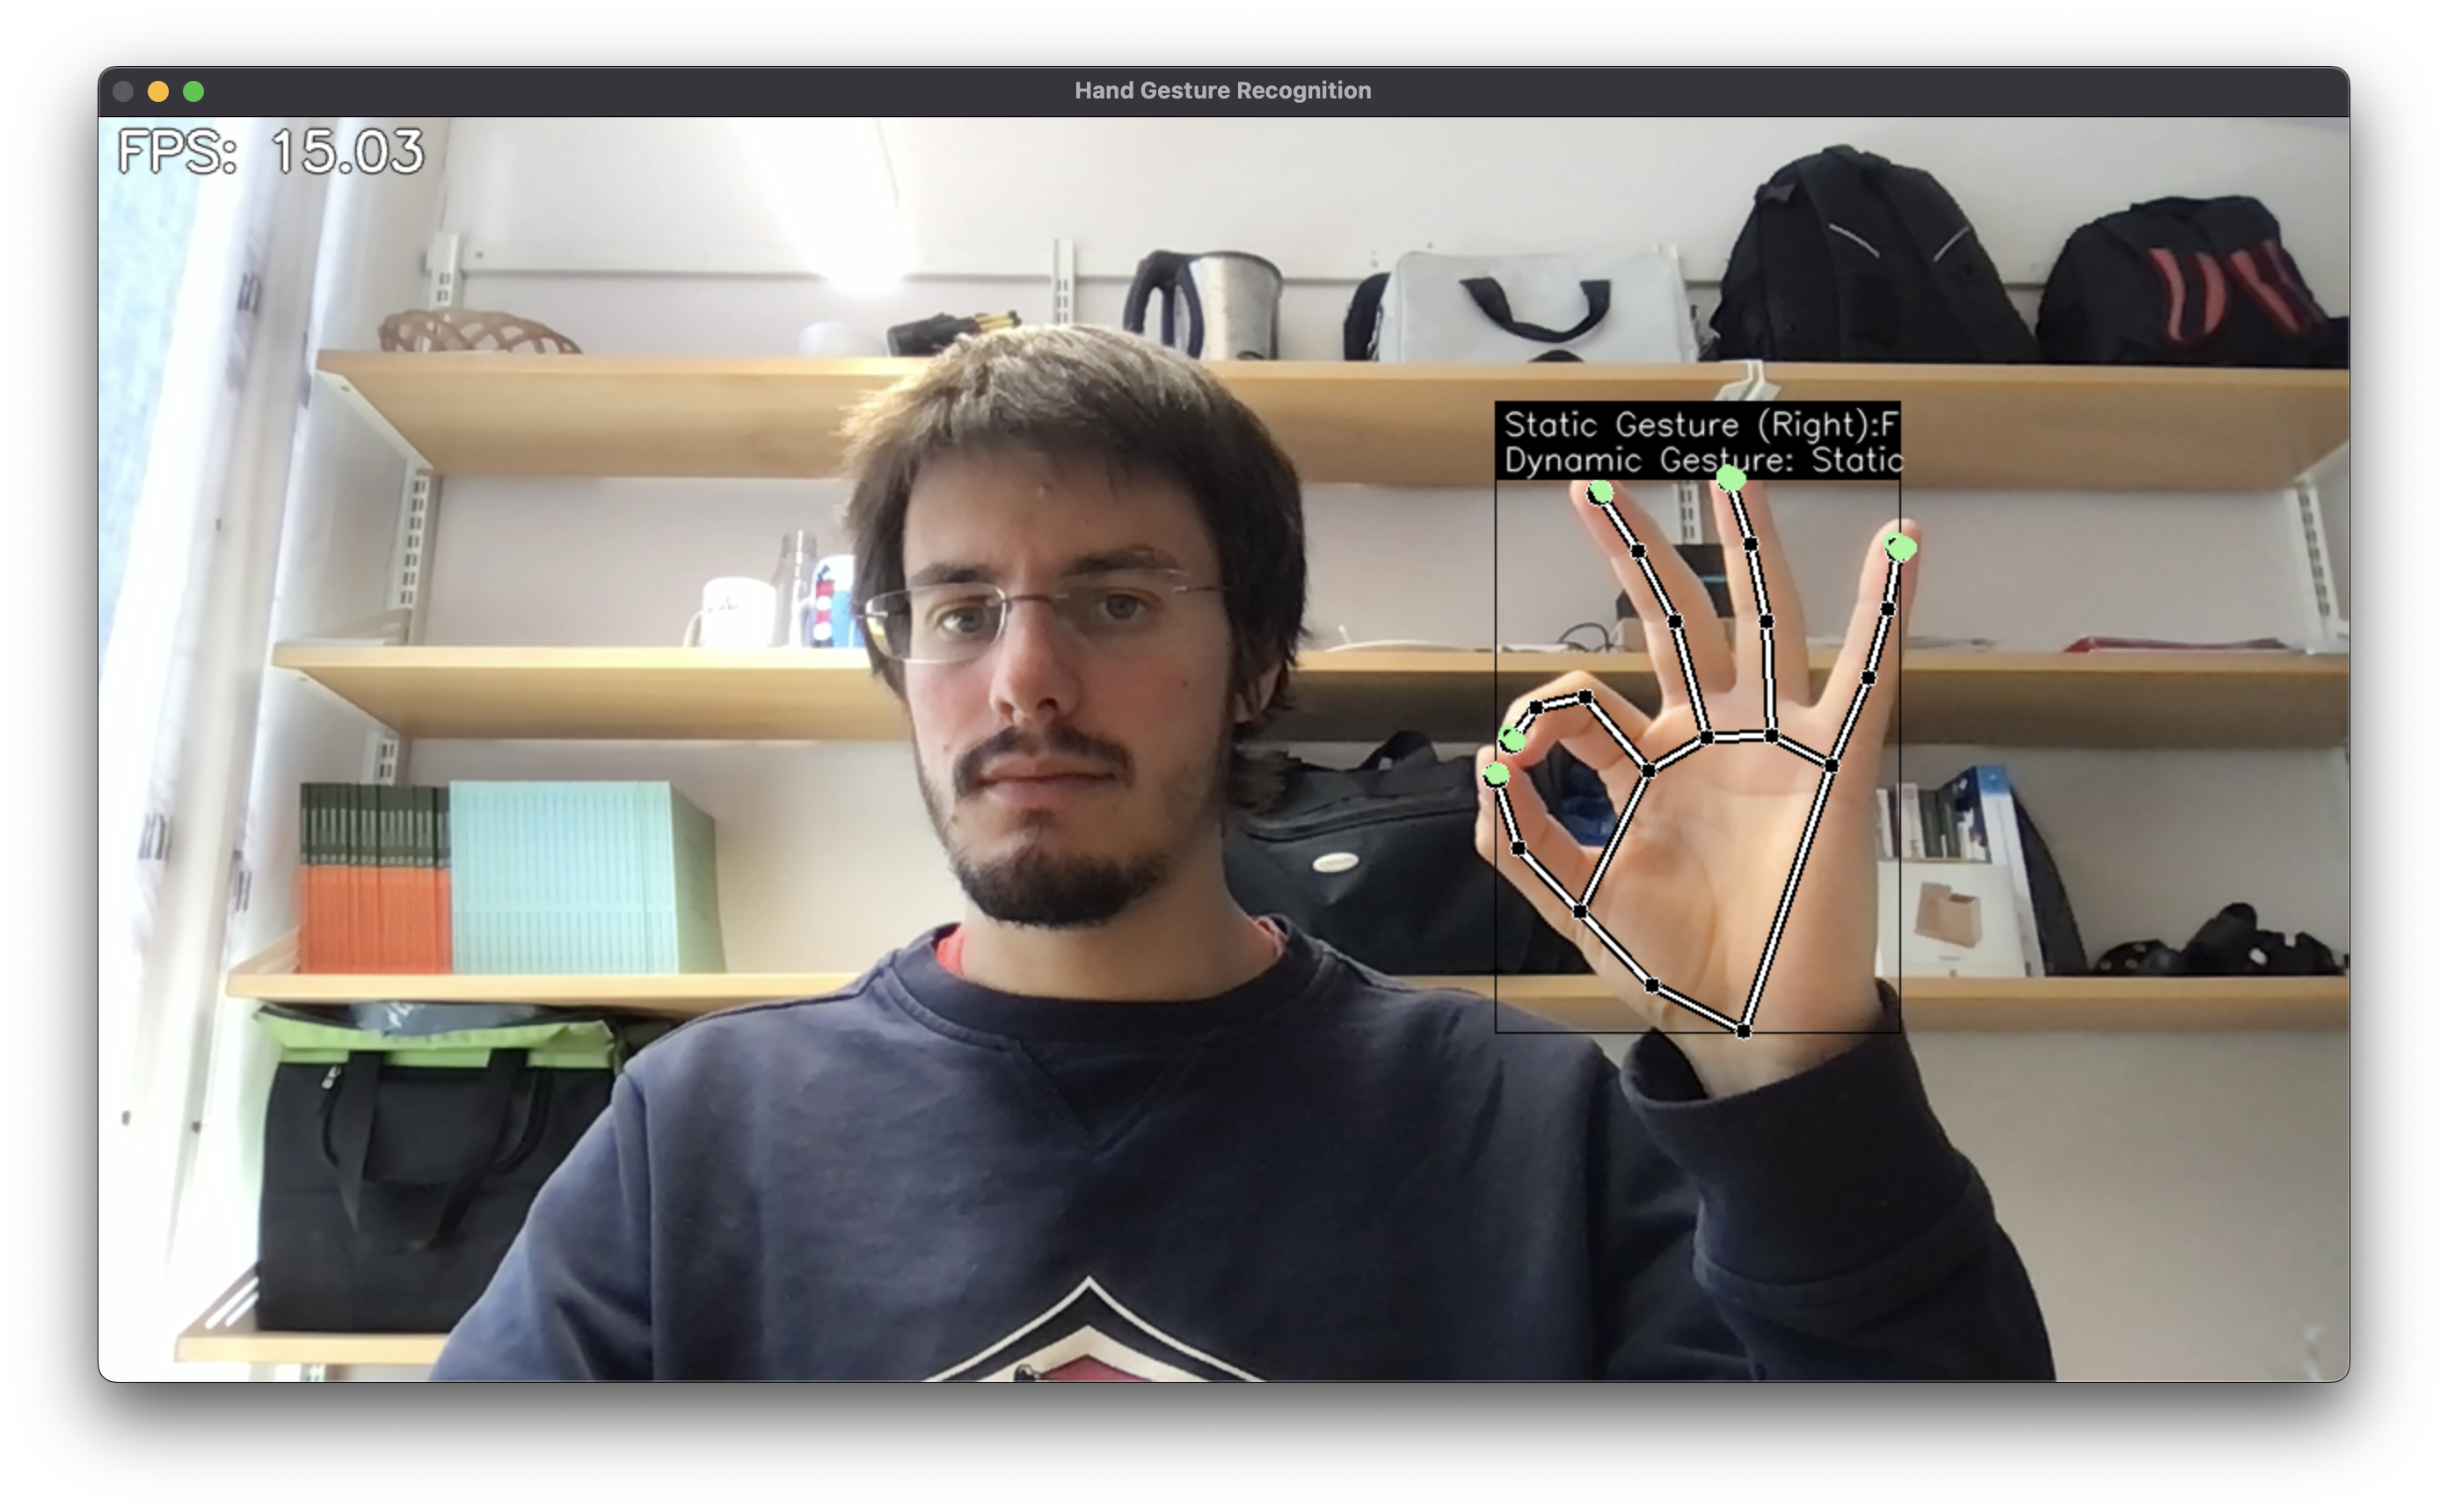
\includegraphics[width=\textwidth]{thesis/images/UI.png}
    \caption{User interface of the program when the webcam is used}
    \label{fig:example_ui}
\end{figure}

\section{Documentation}
To make the system as understandable as possible a proper documentation has been written. To ensure its readiness \textit{MkDocs} has been used with the theme \textit{MkDocs Material} and \textit{Ligthgallery} to manage the images. Instead, to ensure its availability \textit{GitHub Pages} and \textit{GitHub Actions} have been used. In this way it is available for everyone.\footnote{\href{https://jjocram.github.io/hand-gesture/}{https://jjocram.github.io/hand-gesture/}} The documentation explains how to:
\begin{itemize}
    \item setup the environment;
    \item run the simulation;
    \item interact with the program;
    \item understand how the program works. In particular it explains:
    \begin{itemize}
        \item the \texttt{main} function;
        \item the \texttt{GestureDetector} class;
        \item the \texttt{AutomataManager} class;
        \item the \texttt{GestureController} class;
        \item the \texttt{MacroController} class;
        \item the \texttt{MacroRunner} class.
    \end{itemize}
    \item train the neural networks;
\end{itemize}

\section{Data collection}
\subsection{Hand gesture recognizer}
To collect data from the hand gesture recognizer Tensorboard and Tensorflow metrics have been used. Tensorboard has been connected to the train scripts as the documentation explains. Moreover, the evaluation dataset, obtained from both the static hand gestures dataset and the dynamic hand gestures dataset has been exploited to evaluate the trained network on data it has never seen. The data gathered in this way are:
\begin{itemize}
    \item accuracy;
    \item latest loss function value;
    \item time.
\end{itemize}
The time is taken exploiting Python's decorators. Before calling the \texttt{fit} method the time is taken and when the training is finished the time is taken again. The delta between the two times is the time spent for training.

\subsection{System resource utilization}\label{ss:system_resource_utilization}
To collect data while the program is running I wrote a Python script, showed in~\ref{appendix:syste_resource_script}, that launches a process (e.g. the recognizer), collects CPU and RAM usage over time and plots them.

\end{document}
